\documentclass[letterpaper,11pt]{article}

\usepackage{latexsym}
\usepackage[empty]{fullpage}
\usepackage{titlesec}
\usepackage{marvosym}
\usepackage[usenames,dvipsnames]{color}
\usepackage{verbatim}
\usepackage{enumitem}
\usepackage[hidelinks]{hyperref}
\usepackage{fancyhdr}
\usepackage[english]{babel}
\usepackage{tabularx}
\usepackage{fontawesome5}
\usepackage{multicol}
\setlength{\multicolsep}{-3.0pt}
\setlength{\columnsep}{-1pt}
\input{glyphtounicode}

%new packages

\usepackage{fontenc}
\usepackage{amsmath}
\usepackage{amssymb}
\usepackage{graphicx}



%----------FONT OPTIONS----------

\pagestyle{fancy}
\fancyhf{} % clear all header and footer fields
\fancyfoot{}
\renewcommand{\headrulewidth}{0pt}
\renewcommand{\footrulewidth}{0pt}

% Adjust margins
\addtolength{\oddsidemargin}{-0.6in}
\addtolength{\evensidemargin}{-0.5in}
\addtolength{\textwidth}{1.19in}
\addtolength{\topmargin}{-.7in}
\addtolength{\textheight}{1.4in}

\urlstyle{same}

\raggedbottom
\raggedright
\setlength{\tabcolsep}{0in}

% Sections formatting
\titleformat{\section}{
  \vspace{-4pt}\scshape\raggedright\large\bfseries
}{}{0em}{}[\color{black}\titlerule \vspace{-5pt}]



% Ensure that generate pdf is machine readable/ATS parsable
\pdfgentounicode=1

%-------------------------
% Custom commands
\newcommand{\resumeItem}[1]{
  \item\small{
    {#1 \vspace{-2pt}}
  }
}

\newcommand{\classesList}[4]{
    \item\small{
        {#1 #2 #3 #4 \vspace{-2pt}}
  }
}

\newcommand{\resumeSubheading}[4]{
  \vspace{-2pt}\item
    \begin{tabular*}{1.0\textwidth}[t]{l@{\extracolsep{\fill}}r}
      \textbf{#1} & \textbf{\small #2} \\
      \textit{\small#3} & \textit{\small #4} \\
    \end{tabular*}\vspace{-7pt}
}

\newcommand{\resumeSubSubheading}[2]{
    \item
    \begin{tabular*}{0.97\textwidth}{l@{\extracolsep{\fill}}r}
      \textit{\small#1} & \textit{\small #2} \\
    \end{tabular*}\vspace{-7pt}
}

\newcommand{\resumeProjectHeading}[2]{
    \item
    \begin{tabular*}{1.001\textwidth}{l@{\extracolsep{\fill}}r}
      \small#1 & \textbf{\small #2}\\
    \end{tabular*}\vspace{-7pt}
}


\newcommand{\resumeSubItem}[1]{\resumeItem{#1}\vspace{-4pt}}

\renewcommand\labelitemi{$\vcenter{\hbox{\tiny$\bullet$}}$}
\renewcommand\labelitemii{$\vcenter{\hbox{\tiny$\bullet$}}$}

\newcommand{\resumeSubHeadingListStart}{\begin{itemize}[leftmargin=0.0in, label={}]}
\newcommand{\resumeSubHeadingListEnd}{\end{itemize}}
\newcommand{\resumeItemListStart}{\begin{itemize}}
\newcommand{\resumeItemListEnd}{\end{itemize}\vspace{-5pt}}

\begin{document}
\fontfamily{cmr}\selectfont
\begin{center}
\parbox{3.0cm}{%
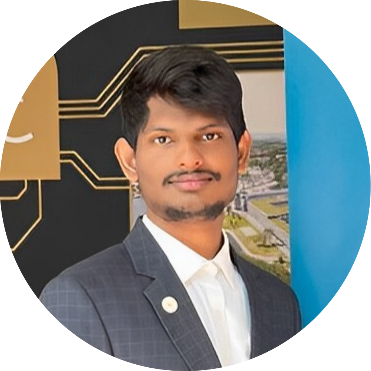
\includegraphics[width=2.7cm,clip]{images/resume_pic_m.png}}
}
\parbox{\dimexpr\linewidth-3.8cm\relax}{
\vspace{-20pt}
\begin{tabularx}{\linewidth}{L r} \\
    {\Huge \scshape  Venkata Sai Yakkshit Reddy Asodi}~
    \href{https://www.cedzlabs.com/yakkshit}{\vspace{1pt}}\\
      Berlin, Germany. \\ \vspace{1pt}
     \small \raisebox{-0.1\height}\faPhone\ +91 8179936156 ~ \href{mailto:saiyakkshit2001@gmail.com}{\raisebox{-0.2\height}\faEnvelope\  {saiyakkshit2001@gmail.com}} ~ 
    \href{https://linkedin.com/in/yakkshit/}{\raisebox{-0.2\height}\faLinkedin\ {yakkshit}}  ~
    \href{https://yakkshit.com/}{\raisebox{-0.2\height}\faGlobe\ {yakkshit.com}}  ~
    \href{https://github.com/yakkshit}{\raisebox{-0.2\height}\faGithub{ yakkshit}}
    \vspace{-8pt}
    
\end{tabularx}
}
\end{center}

\vspace{-23pt}

%-----------SUMMARY-----------
\section{Summary}
Dynamic Data Scientist with a background in developing advanced fraud detection algorithms, personalized recommendation systems, and AI-powered chatbot technologies. Experienced in collaborating with global teams and working on projects like sentiment analysis, image/audio classification, and text analysis. Dedicated to learning and applying cutting-edge techniques to solve complex data science challenges.

%-----------TECHNICAL SKILLS-----------
\section{Technical Skills}
\begin{itemize}[leftmargin=0.15in, label={}]
\small{\item{
\textbf{Languages - }{Python, R, SQL, JavaScript (ES6+), HTML5, CSS3.} \\
\textbf{Data Science Tools - }{Pandas, NumPy, Scikit-learn, TensorFlow, Keras.} \\
\textbf{Visualization - }{Matplotlib, Seaborn, Tableau, PowerBI.} \\
\textbf{Machine Learning - }{Supervised Learning, Unsupervised Learning, Deep Learning.} \\
\textbf{Deployment - }{AWS, Docker, Kubernetes, Azure.}\\
\textbf{Frameworks - }{Flask, Django, React, Next.js.}\\
}}
\end{itemize}

\vspace{-10pt}

%-----------EXPERIENCE-----------
\section{Experience}

\resumeSubHeadingListStart

\resumeSubheading
{Circleup AG}{December 2023 -- July 2024}
  {Lead Full Stack Engineer}{Zurich, Switzerland}\\
\vspace{10pt}
\textbf{Responsibilities:}
\resumeItemListStart
\resumeItem{Developed responsive web applications and machine learning-based features, enhancing user experience for AI-driven services.}
\resumeItem{Collaborated on LLM-TGI-related endpoints and implemented user-centered UI/UX designs, improving application scalability and performance.}
\resumeItemListEnd

\resumeSubheading
{Cedzlabs}{March 2023 -- July 2024}
{Full Stack Developer}{India}\\
\vspace{10pt}
\textbf{Responsibilities:}
\resumeItemListStart
\resumeItem{Worked on intuitive and accessible web applications with an emphasis on data visualization and user interaction.}
\resumeItem{Optimized project delivery through Agile methodologies, contributing to scalable cloud-based solutions.}
\resumeItemListEnd

\resumeSubHeadingListEnd

%-----------PROJECTS-----------
\section{Projects}

\resumeSubHeadingListStart

\resumeProjectHeading
{\textbf{AI Fraud Detection System} $|$ \emph{Python, TensorFlow, Scikit-learn}}{April 2024}\\
\vspace{5pt}
\resumeItemListStart
\resumeItem{Built a fraud detection system for financial institutions, using machine learning algorithms to detect and prevent fraudulent activities. Achieved 95\% accuracy using ensemble learning models.}
\resumeItemListEnd

\resumeProjectHeading
{\textbf{Sentiment Analysis for E-commerce Reviews} $|$ \emph{Python, NLP}}{January 2024}\\
\vspace{5pt}
\resumeItemListStart
\resumeItem{Developed a sentiment analysis tool that processes customer reviews, identifying sentiment trends and product feedback. Integrated the solution into e-commerce platforms.}
\resumeItemListEnd

\resumeProjectHeading
{\textbf{Personalized Recommendation System} $|$ \emph{Python, Flask, AWS}}{July 2024}\\
\vspace{5pt}
\resumeItemListStart
\resumeItem{Engineered a recommendation engine for an e-commerce platform, improving product discovery using collaborative filtering and content-based techniques.}
\resumeItemListEnd

\resumeSubHeadingListEnd

%-----------ACHIEVEMENTS-----------
\section{Achievements / Extracurricular}

\resumeSubHeadingListStart
\resumeItemListStart
\resumeItem{Successfully implemented a machine learning model achieving 95\% accuracy in fraud detection.}
\resumeItem{Contributed to various open-source data science projects, including sentiment analysis and image classification.}
\resumeItem{Led a team in a global hackathon to develop an AI chatbot for customer support, winning second place.}
\resumeItemListEnd
\resumeSubHeadingListEnd

\end{document}